\documentclass{beamer}
\usepackage[utf8]{inputenc}
\usepackage{hyperref}
\usepackage{multicol}
\usepackage{hyperref}
\usepackage{amsmath}
\usepackage[english]{babel}
\usepackage{algorithm}
\usepackage[noend]{algpseudocode}

\inputencoding{utf8}

\mode<presentation> {
    \usetheme{Madrid}
}

\usepackage{graphicx}
\usepackage{booktabs}

\title[Quicksort]{Quicksort}
\author{Ernesto Rodriguez - Juan Roberto Alvaro Saravia}
\institute{
    Universidad Francisco Marroquin \\
    \medskip \textit{ernestorodriguez@ufm.edu - juanalvarado@ufm.edu}
}

\date[\today]{}

\begin{document}

\begin{frame}
\titlepage
\end{frame}

\begin{frame}
\frametitle{Quicksort}
\begin{itemize}
    \item{Tiene tiempo de ejecuci\'on de $\mathcal{O}(n^2)$}
    \item{Teoricamente, no es el algoritmo m\'as eficiente}
    \item{Es a menudo la mejor opcion en practica}
    \item{Puede ordenar los arreglos eficientemente \emph{en la misma memoria} (in-place)}
    \item{Su tiempo promedio es $\mathcal{O}(nlog(n))$ y las constantes escondidas son
    peque\~nas.}
    \item{Es el algoritmo de ordenamiento m\'as analizado en la academia y utilizado
    en la industria}
\end{itemize}
\end{frame}

\begin{frame}
\frametitle{Un parentesis}
\begin{itemize}
\item{Algoritmos \emph{in-place} y no \emph{in-place}}
\item{Algoritmos \emph{estables} e \emph{inestables}}
\end{itemize}
\end{frame}

\begin{frame}
\frametitle{Intuici\'on}
Dado un arreglo $Xs$;
\begin{enumerate}
    \item{Seleccionar un indice $p$, llamado pivote}
    \item{Colocar los elementos $x \leq Xs[p]$ a la izquierda del arreglo}
    \item{Colocar los elementos $x > Xs[p]$ a la derecha del arreglo}
    \item{Ordenar recursivamente los arreglos $Xs[1,p-1]$ y $Xs[p+1,\mathtt{len}(Xs)]$}
    \item{Juntar los arreglos resultantes y el pivote en el orden correcto}
\end{enumerate}

\end{frame}

\begin{frame}

\frametitle{Algoritmo}
\begin{algorithm}[H]
    \caption{Quicksort}
    \begin{algorithmic}[1]
    \Procedure{quicksort}{$Ns$,$p$,$r$}
    \If{$p<r$}
        \State{$q\gets \mathtt{particion}(Ns,p,r)$}
        \State{$\mathtt{quicksort}(Ns,p, q-1)$}
        \State{$\mathtt{quicksort}(Ns,q+1,r)$}
    \EndIf
    \EndProcedure
    \end{algorithmic}
\end{algorithm}

Para ordenar un arreglo, se ejecuta: $\mathtt{quicksort}(Ns,1,\mathtt{len}(Ns))$

\end{frame}

\begin{frame}
\frametitle{Partici\'on}

\end{frame}

\begin{frame}
\frametitle{Partici\'on}

\begin{algorithm}[H]
    \caption{Partici\'on}
    \begin{algorithmic}[1]
    \Procedure{particion}{$Ns$,$p$,$r$}
    \State{$x\gets Ns[r]$}
    \State{$i\gets p-1$}
    \For{$j \gets p$ {\bf to} $r-1$}
    \If{$A[j]\leq x$}
        \State{$i\gets i+1$}
        \State{$\mathtt{intercambiar}(Ns,i,j)$}
    \EndIf
    \EndFor
    \State{$\mathtt{intercambiar}(Ns,i+1,r)$}
    \State \Return{$i+1$}
    \EndProcedure
    \end{algorithmic}
\end{algorithm}
\begin{itemize}
\item{Similitudes entre esta implementaci\'on y la suya}
\item{Analisis asintoticio entre ambos}
\end{itemize}

\end{frame}

\begin{frame}
\frametitle{Partici\'on}
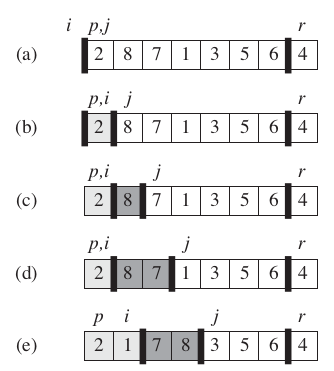
\includegraphics[width=5cm]{particion1.png}
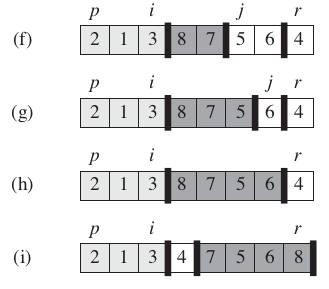
\includegraphics[width=5cm]{particion2.png}
\end{frame}
\end{document}